\documentclass[aspectratio=169]{beamer}

\usepackage[utf8]{inputenc}
\usetheme{Madrid}
\usecolortheme{beaver}
\usepackage{fontspec}
\usepackage{listings}
\usepackage{hyperref}
\usepackage{fancyvrb}

%Information to be included in the title page:
\title{Testing Techniques in Go}
%\subtitle{}
\author{Baiju Muthukadan}
\institute{Red Hat}
\date{@nogenerics}

\logo{
\includegraphics[height=1.5cm]{images/gopher.jpg}}

\begin{document}
\beamertemplatenavigationsymbolsempty

\setmainfont
[ Path = fonts/,
UprightFont = DejaVuSerif.ttf,
ItalicFont = DejaVuSerif-Italic.ttf,
BoldFont = DejaVuSerif-Bold.ttf,
BoldItalicFont = DejaVuSerif-BoldItalic.ttf,
Numbers={Lining, Monospaced},
] {DejaVu Serif}

\setsansfont
[ Path = fonts/,
UprightFont = DejaVuSans.ttf,
ItalicFont = DejaVuSans-Oblique.ttf,
BoldFont = DejaVuSans-Bold.ttf,
BoldItalicFont = DejaVuSans-BoldOblique.ttf,
Numbers={Lining, Monospaced},
] {DejaVu Sans}

\setmonofont
[ Path = fonts/,
UprightFont = DejaVuSansMono.ttf,
ItalicFont = DejaVuSansMono-Oblique.ttf,
BoldFont = DejaVuSansMono-Bold.ttf,
BoldItalicFont = DejaVuSansMono-BoldOblique.ttf,
Numbers={Lining, Monospaced},
] {DejaVu Sans Mono}


\newfontfamily{\vollkorn}
[ Path = fonts/,
UprightFont = Vollkorn-Regular.otf,
ItalicFont = Vollkorn-Italic.otf,
BoldFont = Vollkorn-Bold.otf,
BoldItalicFont = Vollkorn-BoldItalic.otf,
Numbers={Lining, Monospaced},
] {Vollkorn}

\newfontfamily{\dejavuserif}
[ Path = fonts/,
UprightFont = DejaVuSerif.ttf,
ItalicFont = DejaVuSerif-Italic.ttf,
BoldFont = DejaVuSerif-Bold.ttf,
BoldItalicFont = DejaVuSerif-BoldItalic.ttf,
Numbers={Lining, Monospaced},
] {DejaVu Serif}

\newfontfamily{\dejavusans}
[ Path = fonts/,
UprightFont = DejaVuSans.ttf,
ItalicFont = DejaVuSans-Oblique.ttf,
BoldFont = DejaVuSans-Bold.ttf,
BoldItalicFont = DejaVuSans-BoldOblique.ttf,
Numbers={Lining, Monospaced},
] {DejaVu Sans}

\newfontfamily{\dejavumono}
[ Path = fonts/,
UprightFont = DejaVuSansMono.ttf,
ItalicFont = DejaVuSansMono-Oblique.ttf,
BoldFont = DejaVuSansMono-Bold.ttf,
BoldItalicFont = DejaVuSansMono-BoldOblique.ttf,
Numbers={Lining, Monospaced},
] {DejaVu Sans Mono}

\frame{\titlepage}

\begin{frame}
  \frametitle{About Me}

  \begin{itemize}
  \item<1-> Senior Software Engineer, Red Hat
  \item<2-> FOSS Contributor (SMC, Koha, Zope, SaltStack, fabric8 etc.)
  \item<3-> Founded the Swathanthra Malayalam Computing (SMC) project in 2001 while studying at REC Calicut (NIT Kozhikode)
  \item<4-> Received the first Kenneth Gonsalves Award for contributions to the Python community in India
  \item<5-> Author of the book: A Comprehensive Guide to Go Programming \footnote{\url{https://golang.muthukadan.net}}
  \end{itemize}

\end{frame}

\begin{frame}
  \frametitle{Test what you fly, fly what you test!}

  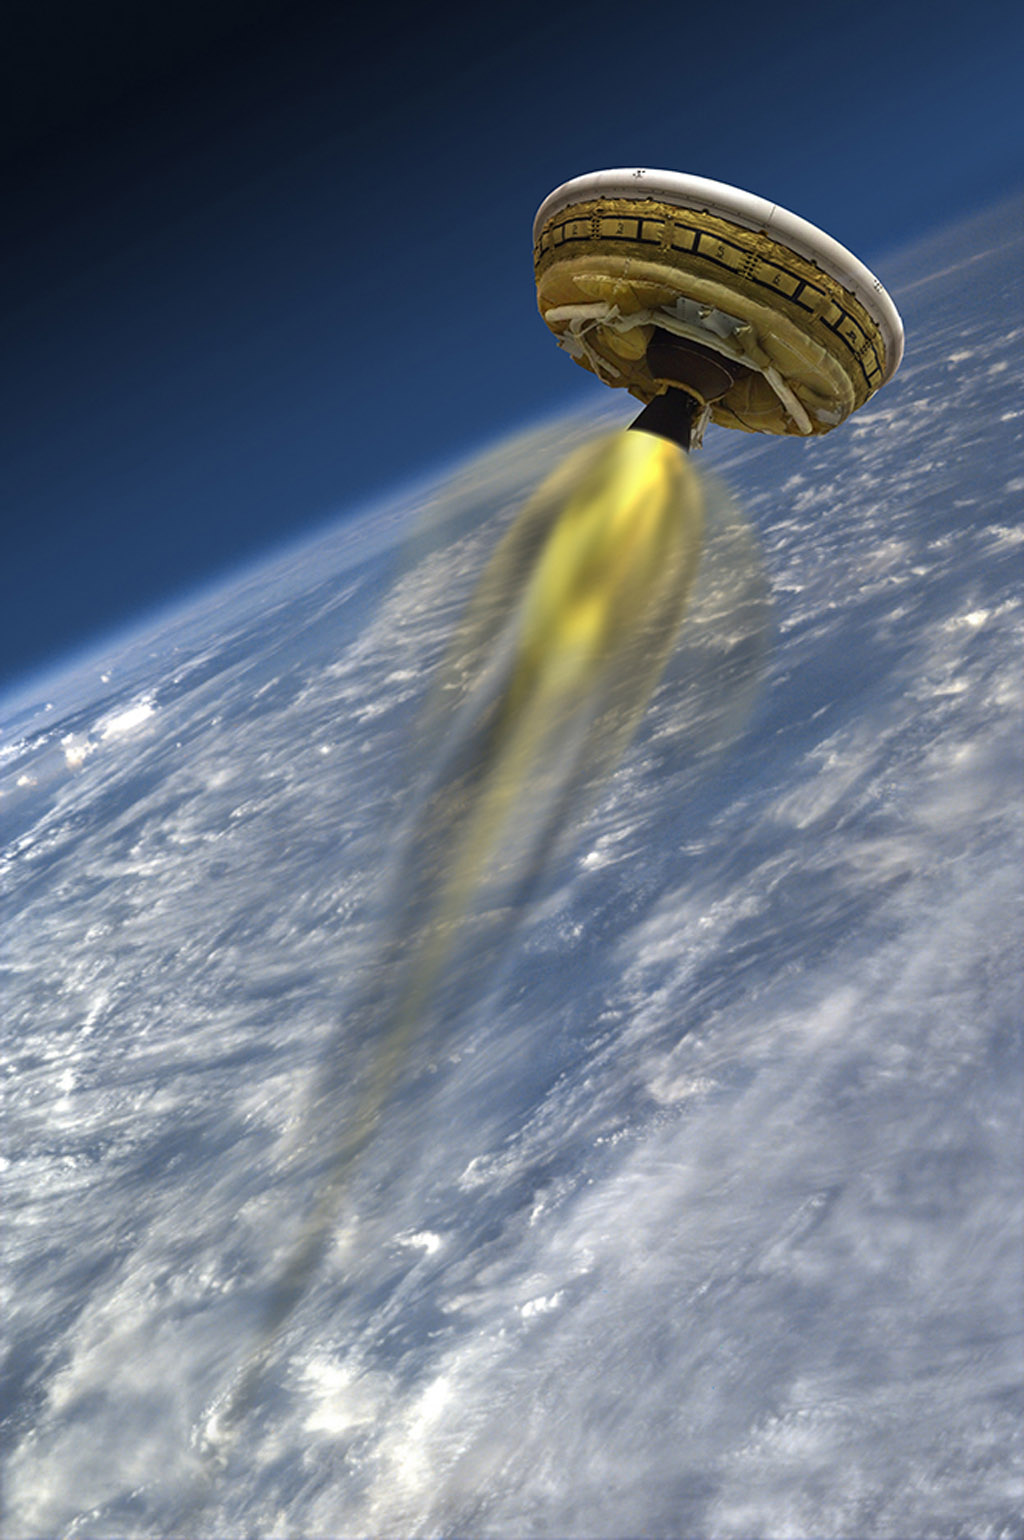
\includegraphics[scale=.35]{images/PIA18017_hires.jpg}
  %% https://en.wikipedia.org/wiki/Low-Density_Supersonic_Decelerator
  
\end{frame}

\begin{frame}[fragile]
  \frametitle{go test}

  \begin{lstlisting}
    go test -v
    go test ./some-package -v
    go test ./some-package -v -run TestPattern
    go test ./some-package -v -cover
  \end{lstlisting}
  
  \url{https://golang.org/cmd/go/\#hdr-Test\_packages}
  
\end{frame}

\begin{frame}[fragile]
  \frametitle{File: hello\_test.go}

  \lstinputlisting{hello/hello_test.go}
  
\end{frame}


\begin{frame}[fragile]
  \frametitle{File: hello.go}

  \lstinputlisting{hello/hello.go}
  
\end{frame}


\begin{frame}%%     1
\begin{center}
{\huge Thank You!}\\[1cm]
{\large \href{https://twitter.com/nogenerics}{@nogenerics}}
\end{center}
\end{frame}

\end{document}
